{\color{indiagreen}\subsection{Integracija v Unity-ju}}
Unity ponuja že v samem editorju dva različna version control sistema. To sta Perforce(\url{https://www.perforce.com/}) in Plastic SCM(\url{https://www.plasticscm.com/}). Sedaj se pojavi tudi vprašanje zakaj bi uporabljali kateri koli version control sistem. Ena izmed ključnih lastnosti je, da lahko spremljamo potek sprememb in da se lahko kadarkoli v procesu vrnemo na prejšnjo rešitev. Da nam pa tudi funkcije, kot npr. kdo v ekipi je naredil spremembo, kakšne so spremembe med samimi spremembami (commit-i) in lažje vidimo kje so nastale napake ali hrošči. 
V moji seminarski nalogi ne bom uporabljal teh dveh orodji, ampak bom uporabljal čisto osnovni GIT, kot stran oz. server kjer bo držal bo uporabil GitHub(\url{https://github.com/}). 
Najprej bomo seveda nastavili Unity tako, da bomo lahko primerjali datoteke med seboj. To naredimo tako da \textbf{Edit} $\rightarrow$ \textbf{Project Settings} $\rightarrow$ \textbf{Editor menu}. Tukaj nastavimo, da se vse datoteke nujno spremenijo v .txt datoteke.\\
\begin{figure}[ht!]
	\centering
	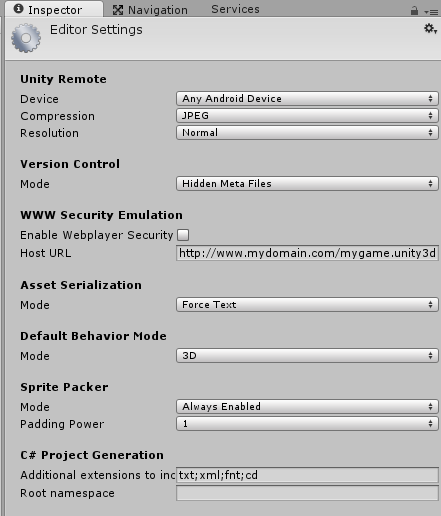
\includegraphics[width=9cm, height=12cm,keepaspectratio=true]{VersionControl.png}
	\caption{Namestitev version control}
\end{figure}
Saj ima Unity po primarnih (default) nastavitvah nekatere objekte zapisane v binarnem sistemu, pri katerih je skoraj nemogoče spremljati spremembe.